\documentclass[./SoftwareEngineering.tex]{subfiles}

\section*{Lởi mở đầu}
\addcontentsline{toc}{section}{Lởi mở đầu}

\begin{wrapfigure}{r}{0.25\textwidth}
	\centering
	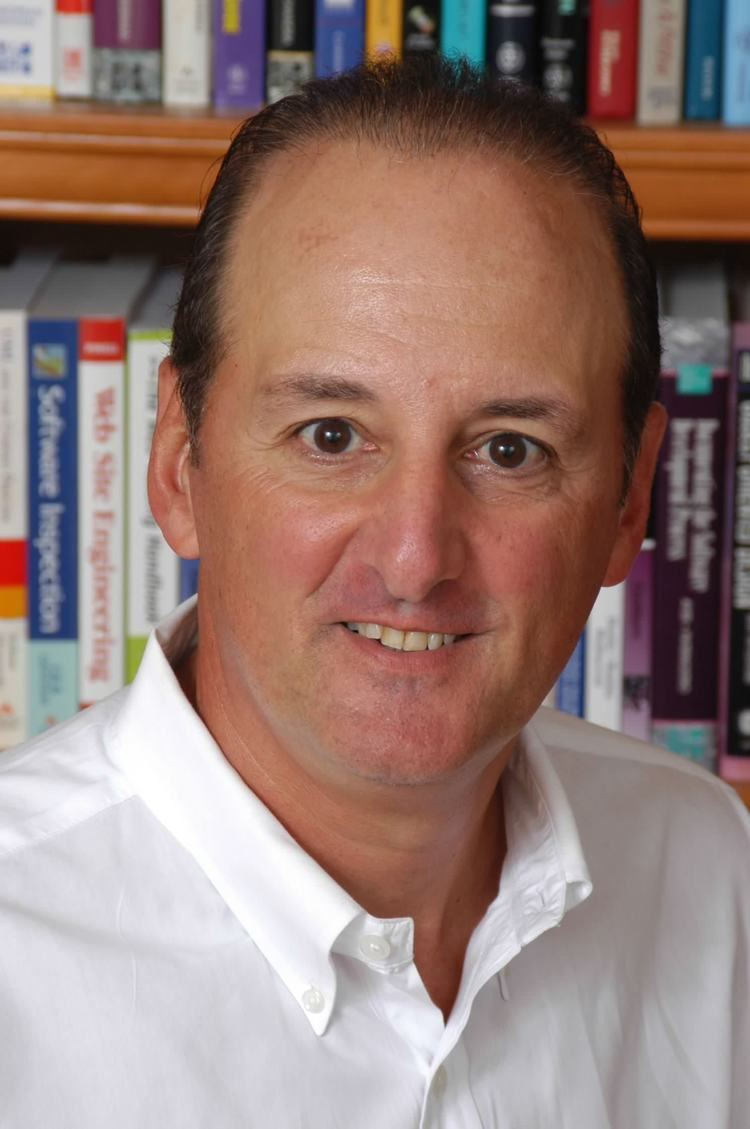
\includegraphics[width=0.9\linewidth]{./images/Pressman.png}
\end{wrapfigure}

\textbf{Tiến sĩ Roger S. Pressman} không những là một kỹ sư phần mềm nổi tiếng, một nhà tư vấn giỏi mà còn là một giáo sư nhiều kinh nghiệm trong ngành sư phạm. Với hơn 40 năm hoạt động trong lĩnh vực kỹ nghệ phần mềm, ông đã viết nên cuốn sách \textit{“Software Engineering A Practitioner's Approach”} nhằm giải quyết tất cả những vấn đề thường gặp từ đơn giản đến phức tạp liên quan đến kỹ nghệ phần mềm. Các nội dung trong sách đã được tác giả trình bày một cách hệ thống, khoa học và mang tính sư phạm cao. Đây là cuốn sách phù hợp với tất cả sinh viên CNTT cũng như những người làm việc trong lĩnh vực kỹ nghệ phần mềm.

Quá trình xây dựng nên một phần mềm tốt phải trải qua rất nhiều bước, mỗi bước lại chiếm một vai trò nhất định trong quá trình ấy.Trong đó, không thể không kể đến vai trò của bước thiết kế. Thiết kế cũng giống như các công việc khác, muốn hoàn thành tốt thì chúng ta phải có một nền tảng vững chắc, một cái nhìn từ tổng quan rồi mới đến chi tiết.Chính vì vậy, để nắm chắc các khái niệm cơ bản của thiết kế ngay từ bước đầu, nhóm dịch đã quyết định cùng nhau tìm hiểu và nghiên cứu nội dung “Design Concepts” (chapter 8) của cuốn sách. Chương đã giúp các thành viên trong nhóm tiếp cận làm quen với các khái niệm mới, hiểu rõ hơn về các khái niệm cũ và làm rõ hơn nữa tầm quan trọng của việc áp dụng các khái niệm nền tảng ấy vào thiết kế phần mềm.

Do đứng dưới cái nhìn là sinh viên đang tham gia học tập, tìm hiểu về môn Công nghệ phần mềm nên bản dịch chắc chắn có sai sót và chưa chính xác hoàn toàn với bản chính. Và với mong muốn không làm mất ý của tác giả muốn truyền đạt nên nhóm xin phép sẽ không dịch, lược dịch hoặc dịch nhưng sẽ ghi chú kèm từ/câu gốc một số phần để đảm bảo nội dung gốc của tác giả. Mong thầy và các bạn đọc xin ý kiến chỉnh sửa phù hợp với nội dung của tác giả. 
 \begin{flushright}\textbf{Nhóm sinh viên,} \end{flushright} 